\documentclass{standalone}
\usepackage{tikz}
\usetikzlibrary{patterns, positioning}
\usepackage[sfdefault]{ClearSans} %% option 'sfdefault' activates Clear Sans as the default text font
\usepackage[T1]{fontenc}

\begin{document}
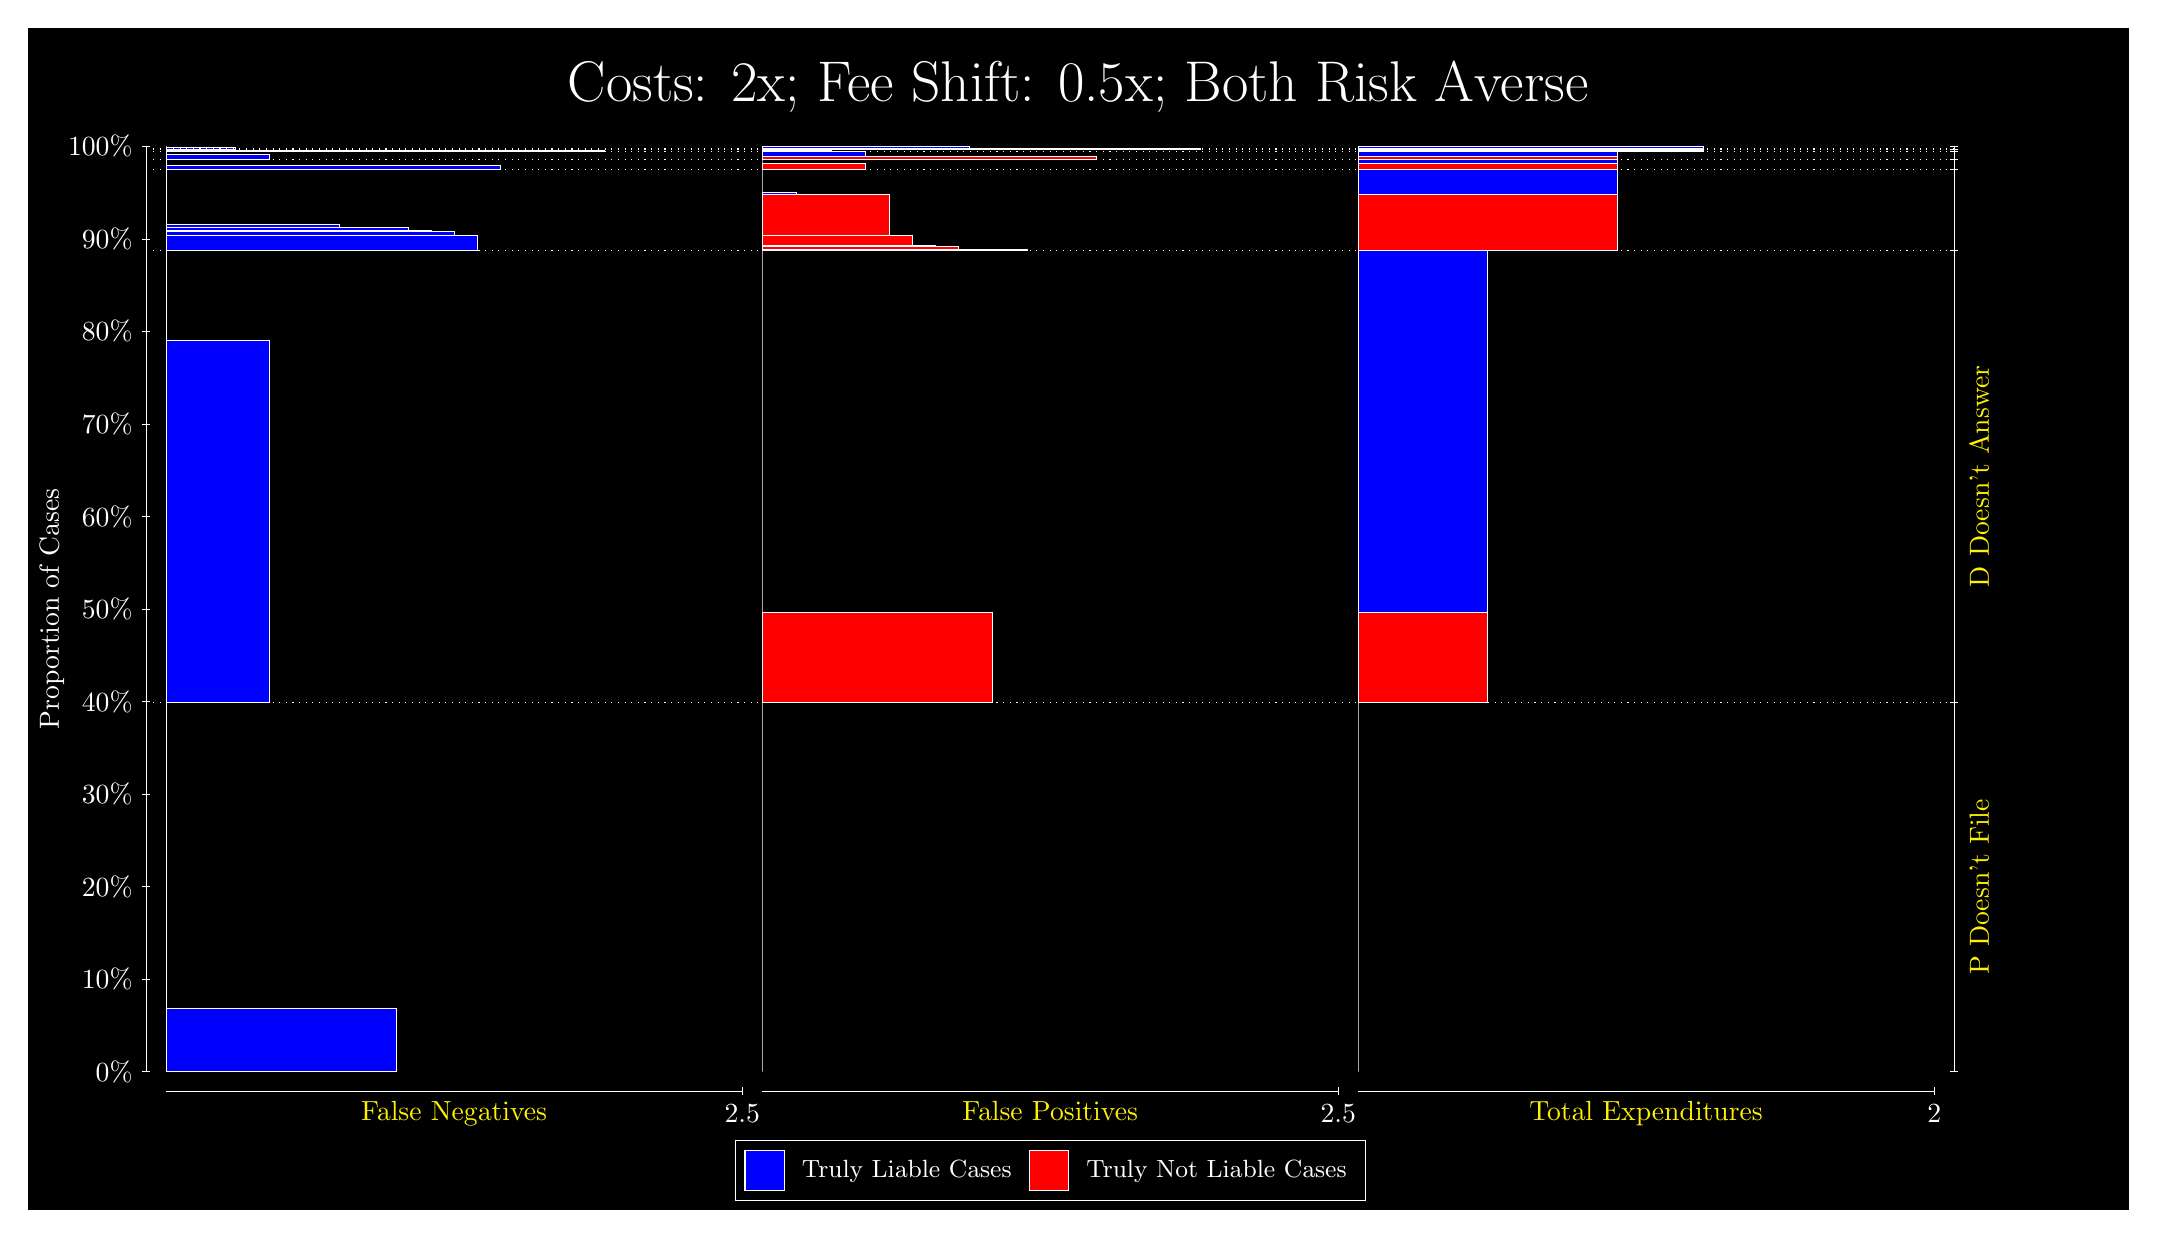
\begin{tikzpicture}
\draw[fill=black] (0,0) rectangle (26.667,15);
\draw[text=white] (0,13.5) rectangle (26.667,15) node[midway] {\huge Costs: 2x; Fee Shift: 0.5x; Both Risk Averse};
\draw[white, very thin] (1.5,1.75) -- (1.5,13.5);
\node[rotate=90, text=white, anchor=center] at (0.3, 7.625) {Proportion of Cases};
\draw[white, very thin] (1.45,1.75) -- (1.55,1.75);
\node[text=white, anchor=east] at (1.45, 1.75) {0\%};
\draw[white, very thin] (1.45,2.925) -- (1.55,2.925);
\node[text=white, anchor=east] at (1.45, 2.925) {10\%};
\draw[white, very thin] (1.45,4.1) -- (1.55,4.1);
\node[text=white, anchor=east] at (1.45, 4.1) {20\%};
\draw[white, very thin] (1.45,5.275) -- (1.55,5.275);
\node[text=white, anchor=east] at (1.45, 5.275) {30\%};
\draw[white, very thin] (1.45,6.45) -- (1.55,6.45);
\node[text=white, anchor=east] at (1.45, 6.45) {40\%};
\draw[white, very thin] (1.45,7.625) -- (1.55,7.625);
\node[text=white, anchor=east] at (1.45, 7.625) {50\%};
\draw[white, very thin] (1.45,8.8) -- (1.55,8.8);
\node[text=white, anchor=east] at (1.45, 8.8) {60\%};
\draw[white, very thin] (1.45,9.975) -- (1.55,9.975);
\node[text=white, anchor=east] at (1.45, 9.975) {70\%};
\draw[white, very thin] (1.45,11.15) -- (1.55,11.15);
\node[text=white, anchor=east] at (1.45, 11.15) {80\%};
\draw[white, very thin] (1.45,12.325) -- (1.55,12.325);
\node[text=white, anchor=east] at (1.45, 12.325) {90\%};
\draw[white, very thin] (1.45,13.5) -- (1.55,13.5);
\node[text=white, anchor=east] at (1.45, 13.5) {100\%};

\draw[white, very thin] (24.457,1.75) -- (24.457,13.5);
\draw[white, very thin] (24.407,1.75) -- (24.507,1.75);
\node[anchor=west] at (24.407, 1.75) {};
\draw[white, very thin] (24.407,6.4368) -- (24.507,6.4368);
\node[anchor=west] at (24.407, 6.4368) {};
\draw[white, very thin] (24.407,12.182) -- (24.507,12.182);
\node[anchor=west] at (24.407, 12.182) {};
\draw[white, very thin] (24.407,13.21) -- (24.507,13.21);
\node[anchor=west] at (24.407, 13.21) {};
\draw[white, very thin] (24.407,13.336) -- (24.507,13.336);
\node[anchor=west] at (24.407, 13.336) {};
\draw[white, very thin] (24.407,13.437) -- (24.507,13.437);
\node[anchor=west] at (24.407, 13.437) {};
\draw[white, very thin] (24.407,13.466) -- (24.507,13.466);
\node[anchor=west] at (24.407, 13.466) {};
\draw[white, very thin] (24.407,13.5) -- (24.507,13.5);
\node[anchor=west] at (24.407, 13.5) {};

\draw[white, very thin, fill=blue] (1.75,1.75) rectangle (4.6775,2.5583);
\draw[white, very thin, fill=red] (1.75,2.5583) rectangle (1.75,6.4368);
\draw[white, very thin, fill=blue] (1.75,6.4368) rectangle (3.0674,11.033);
\draw[white, very thin, fill=red] (1.75,11.033) rectangle (1.75,12.182);
\draw[white, very thin, fill=blue] (1.75,12.182) rectangle (5.7022,12.368);
\draw[white, very thin, fill=blue] (1.75,12.368) rectangle (5.4094,12.423);
\draw[white, very thin, fill=blue] (1.75,12.423) rectangle (5.1167,12.438);
\draw[white, very thin, fill=blue] (1.75,12.438) rectangle (4.8239,12.472);
\draw[white, very thin, fill=blue] (1.75,12.472) rectangle (4.5312,12.473);
\draw[white, very thin, fill=blue] (1.75,12.473) rectangle (3.9457,12.506);
\draw[white, very thin, fill=red] (1.75,12.506) rectangle (1.75,13.21);
\draw[white, very thin, fill=blue] (1.75,13.21) rectangle (5.9949,13.264);
\draw[white, very thin, fill=red] (1.75,13.264) rectangle (1.75,13.336);
\draw[white, very thin, fill=blue] (1.75,13.336) rectangle (3.0674,13.395);
\draw[white, very thin, fill=red] (1.75,13.395) rectangle (1.75,13.437);
\draw[white, very thin, fill=blue] (1.75,13.437) rectangle (7.3123,13.448);
\draw[white, very thin, fill=red] (1.75,13.448) rectangle (1.75,13.466);
\draw[white, very thin, fill=blue] (1.75,13.466) rectangle (2.6283,13.489);
\draw[white, very thin, fill=red] (1.75,13.489) rectangle (1.75,13.5);
\draw[white, very thin, fill=red] (9.3189,1.75) rectangle (9.3189,5.6285);
\draw[white, very thin, fill=blue] (9.3189,5.6285) rectangle (9.3189,6.4368);
\draw[white, very thin, fill=red] (9.3189,6.4368) rectangle (12.246,7.5862);
\draw[white, very thin, fill=blue] (9.3189,7.5862) rectangle (9.3189,12.182);
\draw[white, very thin, fill=red] (9.3189,12.182) rectangle (12.686,12.194);
\draw[white, very thin, fill=red] (9.3189,12.194) rectangle (12.1,12.195);
\draw[white, very thin, fill=red] (9.3189,12.195) rectangle (11.807,12.229);
\draw[white, very thin, fill=red] (9.3189,12.229) rectangle (11.515,12.244);
\draw[white, very thin, fill=red] (9.3189,12.244) rectangle (11.222,12.364);
\draw[white, very thin, fill=red] (9.3189,12.364) rectangle (10.929,12.886);
\draw[white, very thin, fill=blue] (9.3189,12.886) rectangle (9.758,12.92);
\draw[white, very thin, fill=blue] (9.3189,12.92) rectangle (9.3189,13.21);
\draw[white, very thin, fill=red] (9.3189,13.21) rectangle (10.636,13.282);
\draw[white, very thin, fill=blue] (9.3189,13.282) rectangle (9.3189,13.336);
\draw[white, very thin, fill=red] (9.3189,13.336) rectangle (13.564,13.378);
\draw[white, very thin, fill=blue] (9.3189,13.378) rectangle (10.636,13.437);
\draw[white, very thin, fill=red] (9.3189,13.437) rectangle (10.197,13.456);
\draw[white, very thin, fill=blue] (9.3189,13.456) rectangle (9.3189,13.466);
\draw[white, very thin, fill=red] (9.3189,13.466) rectangle (14.881,13.477);
\draw[white, very thin, fill=blue] (9.3189,13.477) rectangle (11.954,13.5);
\draw[white, very thin, fill=red] (16.888,1.75) rectangle (16.888,5.6285);
\draw[white, very thin, fill=blue] (16.888,5.6285) rectangle (16.888,6.4368);
\draw[white, very thin, fill=red] (16.888,6.4368) rectangle (18.534,7.5862);
\draw[white, very thin, fill=blue] (16.888,7.5862) rectangle (18.534,12.182);
\draw[white, very thin, fill=red] (16.888,12.182) rectangle (20.181,12.886);
\draw[white, very thin, fill=blue] (16.888,12.886) rectangle (20.181,13.21);
\draw[white, very thin, fill=red] (16.888,13.21) rectangle (20.181,13.282);
\draw[white, very thin, fill=blue] (16.888,13.282) rectangle (20.181,13.336);
\draw[white, very thin, fill=red] (16.888,13.336) rectangle (20.181,13.378);
\draw[white, very thin, fill=blue] (16.888,13.378) rectangle (20.181,13.437);
\draw[white, very thin, fill=red] (16.888,13.437) rectangle (21.279,13.456);
\draw[white, very thin, fill=blue] (16.888,13.456) rectangle (21.279,13.466);
\draw[white, very thin, fill=red] (16.888,13.466) rectangle (21.279,13.477);
\draw[white, very thin, fill=blue] (16.888,13.477) rectangle (21.279,13.5);
\draw[white, dotted] (1.5,6.4368) -- (24.457,6.4368);
\draw[white, dotted] (1.5,12.182) -- (24.457,12.182);
\draw[white, dotted] (1.5,13.21) -- (24.457,13.21);
\draw[white, dotted] (1.5,13.336) -- (24.457,13.336);
\draw[white, dotted] (1.5,13.437) -- (24.457,13.437);
\draw[white, dotted] (1.5,13.466) -- (24.457,13.466);
\draw[white, very thin] (1.75,1.5) -- (9.0689,1.5);
\node[text=yellow, anchor=north] at (5.4094, 1.5) {False Negatives};
\draw[white, very thin] (9.0689,1.45) -- (9.0689,1.55);
\node[text=white, anchor=north] at (9.0689, 1.45) {2.5};

\draw[white, very thin] (9.3189,1.5) -- (16.638,1.5);
\node[text=yellow, anchor=north] at (12.978, 1.5) {False Positives};
\draw[white, very thin] (16.638,1.45) -- (16.638,1.55);
\node[text=white, anchor=north] at (16.638, 1.45) {2.5};

\draw[white, very thin] (16.888,1.5) -- (24.207,1.5);
\node[text=yellow, anchor=north] at (20.547, 1.5) {Total Expenditures};
\draw[white, very thin] (24.207,1.45) -- (24.207,1.55);
\node[text=white, anchor=north] at (24.207, 1.45) {2};

\node[text=yellow, centered, rotate=90] at (24.777, 4.0934) {P Doesn't File};
\node[text=yellow, centered, rotate=90] at (24.777, 9.3094) {D Doesn't Answer};






\draw (12.978300999999998,1.5) node[draw=none] (baseCoordinate) {};
\begin{scope}[align=center]
        \matrix[scale=0.5, draw=white, below=0.5cm of baseCoordinate, nodes={draw}, column sep=0.1cm]{
            \node[rectangle, draw, minimum width=0.5cm, minimum height=0.5cm, fill=blue] {}; &
            \node[draw=none, font=\small, text=white] (B) {Truly Liable Cases}; &
            \node[rectangle, draw, minimum width=0.5cm, minimum height=0.5cm, fill=red] {}; &
            \node[draw=none, font=\small, text=white] (B) {Truly Not Liable Cases}; \\
            };
\end{scope}

\end{tikzpicture}
\end{document}